\documentclass[12pt, a4paper]{memoir} % for a short document
\usepackage[french,english]{babel}

\usepackage [vscale=0.76,includehead]{geometry}                % See geometry.pdf to learn the layout options. There are lots.
%\geometry{a4paper}                   % ... or a4paper or a5paper or ...
%\geometry{landscape}                % Activate for for rotated page geometry
%\OnehalfSpacing
% \setSingleSpace{1.05}
%\usepackage[parfill]{parskip}    % Activate to begin paragraphs with an empty line rather than an indent
\usepackage{graphicx}
\usepackage{amsmath}
\usepackage{fullpage}
\usepackage{mathptmx} % font = times
\usepackage{helvet} % font sf = helvetica
\usepackage[latin1]{inputenc}
\usepackage{relsize}
\usepackage{float}

% Graphics path
\graphicspath{{img/}}

% Custom styles
\headstyles{komalike}
\nouppercaseheads
\chapterstyle{dash}
\makeevenhead{headings}{\sffamily\thepage}{}{\sffamily\leftmark}
\makeoddhead{headings}{\sffamily\rightmark}{}{\sffamily\thepage}
\makeoddfoot{plain}{}{}{} % Pages chapitre.
\makeheadrule{headings}{\textwidth}{\normalrulethickness}
%\renewcommand{\leftmark}{\thechapter ---}
\renewcommand{\chaptername}{\relax}
\renewcommand{\chaptitlefont}{ \sffamily\bfseries \LARGE}
\renewcommand{\chapnumfont}{ \sffamily\bfseries \LARGE}
\setsecnumdepth{subsection}

% Title page formatting -- do not change!
\pretitle{\HUGE\sffamily \bfseries\begin{center}}
\posttitle{\end{center}}
\preauthor{\LARGE  \sffamily \bfseries\begin{center}}
\postauthor{\par\end{center}}

\newcommand{\jury}[1]{%
\gdef\juryB{#1}}
\newcommand{\juryB}{}
\newcommand{\session}[1]{%
\gdef\sessionB{#1}}
\newcommand{\sessionB}{}
\newcommand{\option}[1]{%
\gdef\optionB{#1}}
\newcommand{\optionB}{}

\renewcommand{\maketitlehookd}{%
\vfill{}  \large\par\noindent
\begin{center}\juryB \bigskip\sessionB\end{center}
\vspace{-1.5cm}}
\renewcommand{\maketitlehooka}{%
\vspace{-1.5cm}\noindent
\includegraphics[height=14ex]{logoINP.png}\hfill\raisebox{2ex}{
\includegraphics[height=7ex]{logoUJF.jpg}}\\
\bigskip
\begin{center} \large
Master of Science in Informatics at Grenoble \\
Master Math\'ematiques Informatique - sp\'ecialit\'e Informatique \\
option \optionB  \end{center}\vfill}
% End of title page formatting

\option{$GVR$}
\title{Adpatative point cloud denoising}%\\\vspace{-1ex}\rule{10ex}{0.5pt} \\sub-title}
\author{Jocelyn MEYRON}
\date{ $<$Defense Date$>$} % Delete this line to display the current date
\jury{
Research project performed at $ GIPSA-lab $ \\\medskip
Under the supervision of:\\
ATTALI Dominique, GIPSA-lab\\
M�RIGOT Quentin, Universit� Paris-Dauphine\\\medskip
Defended before a jury composed of:\\
$[$Prof/Dr/Mrs/Mr$]$ $<$first-name last-name$>$\\
$[$Prof/Dr/Mrs/Mr$]$ $<$first-name last-name$>$\\
$[$Prof/Dr/Mrs/Mr$]$ $<$first-name last-name$>$\\
$[$Prof/Dr/Mrs/Mr$]$ $<$first-name last-name$>$\\
}
\session{$June$\hfill 2015}

%%% Title page
\begin{document}
\selectlanguage{english}
\frontmatter
\begin{titlingpage}
\maketitle
\end{titlingpage}
\setlength{\parskip}{-1pt plus 1pt}

% Abstract
\renewcommand{\abstracttextfont}{\normalfont}
\abstractintoc

% English
\begin{abstract}

% TODO
During this internship, we were interested in the denoising of point clouds and
more specifically an adaptive one: the smoothing is more important at a higher
scale. The idea is to move the point cloud in while minimizing an energy. The
energy we considered here was given by the volume of the Minkowski sum of the
point set with a convex polyhedron.

In order to efficiently construct this sum, we had to construct the Voronoi
diagram for a polyhedral norm.

This report is divided as follows: firstly, we will give a detailed
introduction, then we will focus on the state of the art related techniques.
Moreover, we will start by studying the two dimensional case with the $r$-offset
of a point cloud. We will continue by dealing with the 3D case with a polyhedral
norm.

\end{abstract}

\abstractintoc
\renewcommand\abstractname{R\'{e}sum\'{e}}

% Français
\begin{abstract} \selectlanguage{french}

% TODO
Durant ce stage, nous nous sommes intéressés au lissage de nuage de points.

\end{abstract}

\selectlanguage{english}

% vim: set spelllang=en :

\cleardoublepage

\tableofcontents* % the asterisk means that the table of contents itself isn't put into the ToC
\normalsize

\mainmatter
\SingleSpace

\chapter{Introduction}

% TODO

Point cloud smoothing is a well-studied problem: numerous methods exists and
have been proven to work more or less nicely on different kinds of data
(presence of noise...). In this report, we want to tackle the problem of
smoothing while preserving informations such as small details.

More precisely, given a set of points, we want to be able to smooth it by taking
into account the different scales present in it: we want to be able to control
the smoothing such that it is more important in some directions. An example
where this kind of smoothing could be interesting is when we build a 3D scan of
an object: we want to be able to smooth the point cloud while preserving details
(the signature of the author for example).

A lot of smoothing algorithms already exist, some are related to Computer
Vision, some are more based on Computational Geometry techniques:
\begin{itemize}
    \item Gaussian / Laplacian smoothing and all the related filters: adaptive
        filter...
    \item Jet smoothing: a jet is a truncated Taylor expansion. Such jets are
        fitted around points. Jet smoothing operates by projecting the input
        points on an estimated smooth parametric surface (the so-called jet
        surface). Jets are good because they intrinsically contain
        differential information such as normal, curvature...
\end{itemize}

In this report, we will focus on another algorithm which was proposed by
\cite{chambolle2012nonlocal}. Basically, it is a mean curvature flow under an
energy minimization. This energy is related to a non-local curvature.

More formally, let's suppose we have a point cloud in $ \mathbb{R}^d $ made of $
N $ points : $ p_1, \ldots, p_N $, we want to apply an adaptive smoothing on it.
Firstly, we will compute the energy that we want to minimize: $ E(P) = Vol(P + r
K) $ where $ K $ is a chosen convex polyhedron, $ r \in \mathbb{R} $ and $ (+) $
is the Minkowski sum. If we choose $ K = B(0, 1) $ an euclidean ball, then $ P +
rK $ is the $ r $-offset of P and $ E(P) $ is a measure of a union of balls
(like its volume, or the area of its boundary). In this case, the $ r $-offset
will contain intrinsic informations about the point set like normal direction or
curvature approximation.

Secondly, we will need to compute the gradient of this energy. For doing that,
there are multiple choices: use analytical formulae (which exist at least in
2D), use approximations (finite differences) or use a technique called automatic
differentiation that allows use to differentiate any function by changing the
number type and so increasing the complexity a little bit. We will try to use,
in most cases, the automatic differentiation method since it allows us to have
better results than approximate methods without being too painful to implement.

Finally, we will do one step of the flow: move our point set in the direction
which will be computed as the result of a gradient descent algorithm applied on
the point set. The weighting of the gradients will be an important question.

The advantage of such algorithm resides in its anisotropy: since the polyhedron
$ K $ may be any convex polyhedron, it can privilege some directions in the
space and so preserve details in some directions.

We will test this algorithm using multiple polyhedrons, values of $ r
$, point sets with a small / high amount of noise to see if the algorithm is
noise-resilient or not.

% vim: set spelllang=en :

\chapter{State of the art}

% TODO

Nowadays, the traditional methods used for smoothing a point cloud are the
following:
\begin{itemize}
    \item Moving Least Squares (MLS) and its adaptive variant
    \item Laplacian smoothing
\end{itemize}

In this internship, we chose to use a Mean Curvature Flow based technique.

Let's recall the more important results related to the MCF.
First the definition of this flow, given a surface. We want to move each point f
this surface in the direction of its inward normal by an amount related to the
mean curvature at this point.

Multiple approaches exist:
\begin{itemize}
    \item Level-set approach: the moving surface is represented by : $ \{ x |
        \phi(x, t) = 0 \} $. Then $ \phi $ satisfies the following equation: $
        \frac{\partial \phi}{\partial t} = |\nabla \phi| div(\frac{\nabla
            \phi}{| \nabla \phi |}) $.
    \item Graph approach: the surface is a graph of a function $ f : U
        \rightarrow \R $. Then $ f $ satisfies the following equation: $
        \frac{\partial f}{\partial t} = \sqrt{|\nabla f|^2 + 1} ~div(\frac{\nabla
        f}{\sqrt{|\nabla f|^2 + 1}}) $.
\end{itemize}

The MCF is well known for its smoothing properties used for example in image
processing (see \cite{ciomaga2010level}).

We can also relate the MCF to the gradient flow of the surface area functional.

% vim: set spelllang=en :

\chapter{2D case}

\section{Problem}
In this part, we will focus on a 2D point cloud and we will use for the energy
the area of the $ r $-offset of a point cloud $ X $: the Minkowski sum with an euclidean
ball $ B(0, r) $. This offset will be denoted by $ X^{\oplus r} $.

\section{Area of a union of balls}
In order to compute this energy, we need to know how to estimate the area of the
intersection of a ball and a Voronoi cell. Indeed, the area of the union of
balls is the same as the sum of the areas of the restrictions of the balls to
their Voronoi cell (because essentially the Voronoi cells partition the plane).

This is the same work as the one done in \cite{cazals2011computing} except that
we restrict ourselves to 2D which is simpler than in 3D.

For doing that, we need to decompose the intersection into triangles and
spherical caps.

The following figure illustrates the different cases for the intersection of a
Voronoi cell and a ball in 2D:
\begin{figure}[H]
    \centering
    \begin{minipage}{0.32\linewidth}
        \centering
        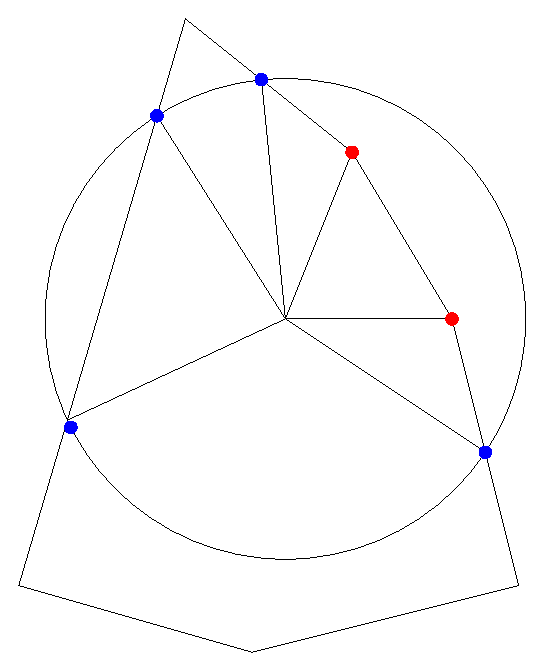
\includegraphics[scale=0.4]{2d/inter_voronoi_ball_2d}
        \subcaption{General case}
        \label{fig:inter_voronoi_ball_2d:a}
    \end{minipage}
    \begin{minipage}{0.32\linewidth}
        \centering
        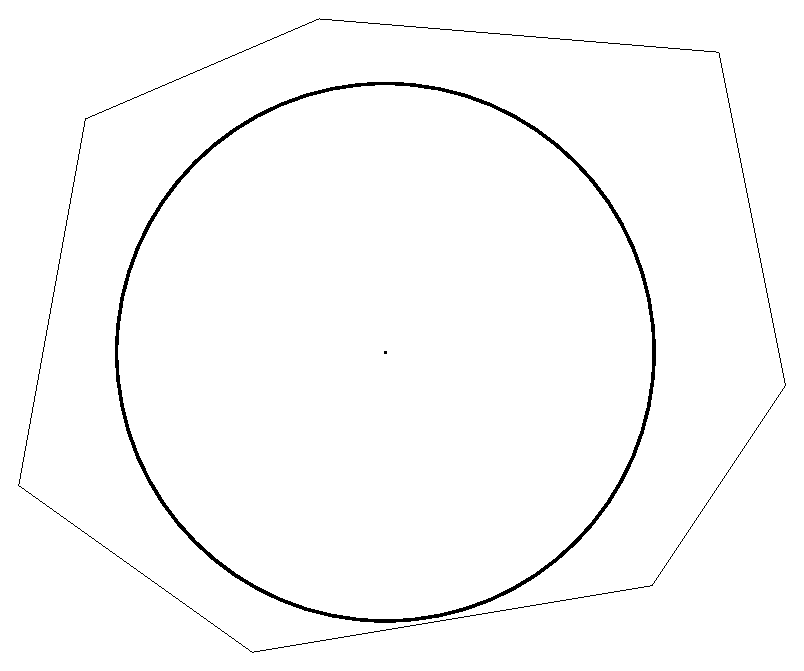
\includegraphics[scale=0.4]{2d/inter_voronoi_ball_2d_no_inter}
        \subcaption{No intersections}
        \label{fig:inter_voronoi_ball_2d:b}
    \end{minipage}
    \begin{minipage}{0.32\linewidth}
        \centering
        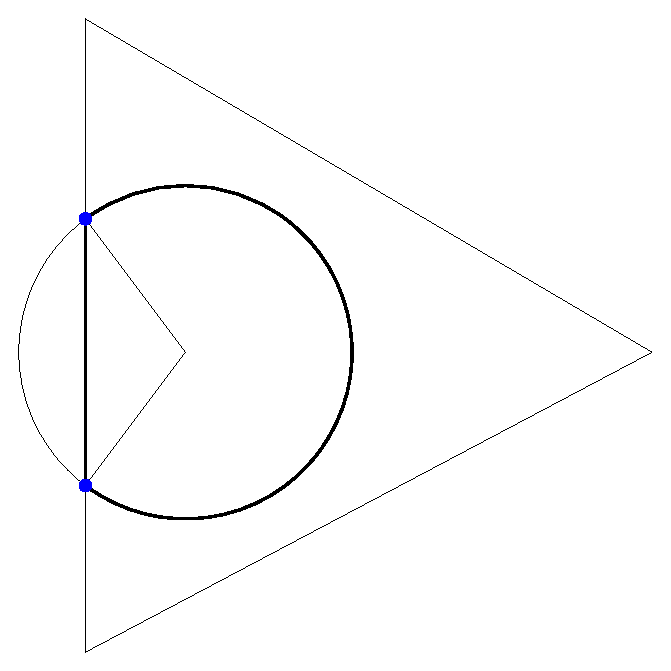
\includegraphics[scale=0.4]{2d/inter_voronoi_ball_2d_2_inter}
        \subcaption{2 intersections}
        \label{fig:inter_voronoi_ball_2d:c}
    \end{minipage}

   \caption{Different cases for the intersection between a Voronoi cell and a sphere}
   \label{fig:inter_voronoi_ball_2d}
\end{figure}

We used \texttt{CGAL} to compute the Delaunay triangulation of our point set.
Given this triangulation, we can compute the Voronoi cell of a point by doing
the following:
\begin{enumerate}
    \item Access the neighbouring faces of a vertex using the
        \texttt{incident\_faces} method.
    \item Compute the Voronoi vertices of these faces using the \texttt{dual}
        method.
\end{enumerate}

Then, we will need to know the vertices of the boundary of the intersection (the
points forming the bold boundary in \ref{fig:inter_voronoi_ball_2d}). There are
two types of those points: some are Voronoi vertices and some are intersections
of Voronoi edges and circles. To each of these points, we attach a boolean
saying whether the point is an interior point or an intersection one. We also
attach the corresponding Voronoi edge.

Then, we loop over the Voronoi edges $ e = pq $ of a vertex $ v $:
\begin{itemize}
    \item if $ p $ and $ q $ are interior points, we add the triangle $ pvq $.
    \item if $ p $ or $ q $ is interior point, we add the triangle $ pvq $.
    \item if $ p $ and $ q $ are intersection points, then if they belong to the
        same Voronoi edge, we add the triangle $ pvq $. If not, we add the
        angular sector $ \vec{vp}, \vec{vq} $.
\end{itemize}

Some special cases need to be handled:
\begin{itemize}
    \item the boundary of the Voronoi cell is entirely outside the ball, then we
        add $ \pi r^2 $ to the area of the union (see
        \ref{fig:inter_voronoi_ball_2d:b}).
    \item the boundary consists of two intersection points $ p $ and $ q $, then
        we add the triangle $ pvq $ and the angular sector $ \vec{vp}, \vec{vq}
        $ (see \ref{fig:inter_voronoi_ball_2d:c}).
    \item there is only one point on the boundary (can happen if adjacent balls
        are tangential), then we add $ \pi r^2 $.
\end{itemize}

We used the same techniques for computing the perimeter of the boundary of the
intersection except that if there are no intersection then the perimeter is null
and instead of adding triangles areas or angular sectors, we add lengths of
circular arcs.

% TODO

\section{Automatic differentiation}

The automatic differentiation is a technique used for computing the derivatives,
gradient of expressions. It is not the same as the symbolic or the numerical
differentiation.

Indeed, automatic differentiation can be used to compute derivatives of programs
and not only mathematical functions without using approximations like with
numerical differentiation.

Let us suppose that we want to compute the derivative of a function $ f $ with a
single one dimensional argument $ x $. To do that, we will replace the number
type that is to say that we will replace $ x $ by $ x + \epsilon x' $ where $
\epsilon $ with the property $ \epsilon^2 = 0 $. Then, we overload all the
arithmetical operations: addition, subtraction, multiplication, division.

Then we call $ f $ with this variable: $ f(x + \epsilon x') = y + \epsilon y'
$. We conclude that $ y = f(x) $ and $ y' = x' f'(x) $ . Indeed for small values
of $ \epsilon $, we have the first order Taylor expansion: $ f(x + \epsilon x') =
f(x) + \epsilon x' f'(x) + ... $. $ x' $ is called a seed and can be chosen
arbitrarily, we can for instance choose $ x ' = 1 $ and so $ y' = f'(x) $.

This process can be easily extended to handle functions like $ f : \R^n
\rightarrow \R $ in order to compute gradients of such functions. This is what
we did: we considered a function over $ n $ points as $ f : \R^{2n} \rightarrow
\R $.

This technique is interesting because it allows us to compute accurate
derivatives of functions very easily and efficiently. Indeed, we only have to
change the number type and write the good implementations of the basic
arithmetic operations.
In \texttt{CGAL}, this is easy to do since the library is already parametrized
by the number type.

% TODO

\section{Gradient}

Then, we used the previously described automatic differentiation technique to
compute the gradient of the previously computed area.

Here are a few examples of such gradients for different input point sets:

\begin{figure}[H]
    \centering

    \begin{minipage}{0.8\linewidth}
        \centering
        \includegraphics[scale=0.3]{2d/area/ellipse-100-01-15}
        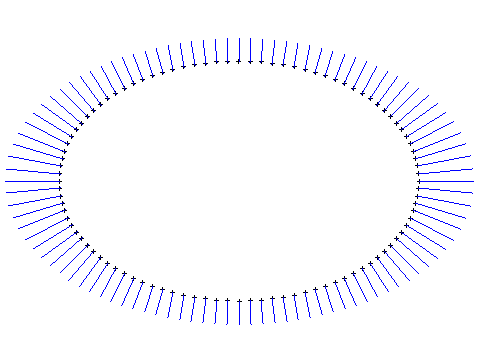
\includegraphics[scale=0.3]{2d/area/ellipse-100-01-15-gradients}
        \subcaption{100 samples on an ellipse with $ r = 15 $}
        \label{fig:gradients_area_2d_ellipse}
    \end{minipage}

    \begin{minipage}{0.8\linewidth}
        \centering
        \includegraphics[scale=0.32]{2d/area/circle-100-01-15}
        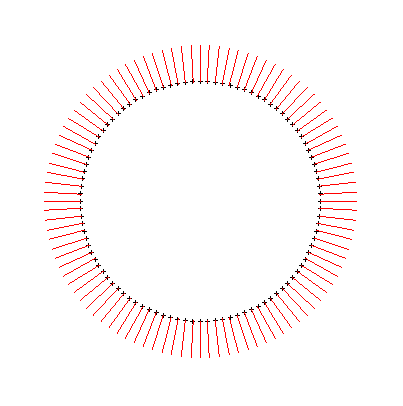
\includegraphics[scale=0.32]{2d/area/circle-100-01-15-gradients}
        \subcaption{100 samples on a circle with $ r = 15 $}
        \label{fig:gradients_area_2d_circle}
    \end{minipage}

    \begin{minipage}{0.8\linewidth}
        \centering
        \includegraphics[scale=0.32]{2d/area/square-76-001-100}
        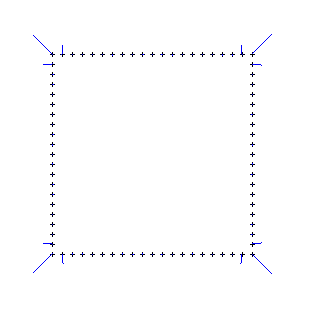
\includegraphics[scale=0.32]{2d/area/square-76-001-100-gradients}
        \subcaption{76 samples on a square with $ r = 100 $}
        \label{fig:gradients_area_2d_square}
    \end{minipage}

    \caption{Input point set / Computed gradients}
    \label{fig:gradients_area_2d}
\end{figure}

We did the same thing using the gradient of the perimeter of the boundary on the
same point clouds.

\begin{figure}[H]
    \centering

    \begin{minipage}{0.8\linewidth}
        \centering
        \includegraphics[scale=0.3]{2d/perimeter/ellipse-100-01-15}
        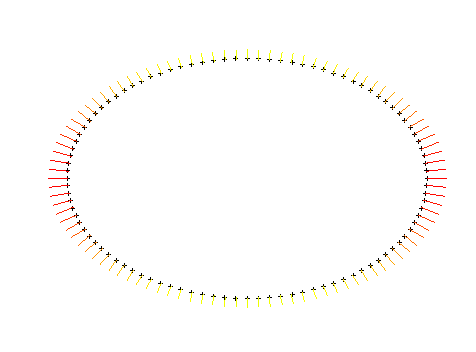
\includegraphics[scale=0.3]{2d/perimeter/ellipse-100-01-15-gradients}
        \subcaption{100 samples on an ellipse with $ r = 15 $}
        \label{fig:gradients_perimeter_2d_ellipse}
    \end{minipage}

    \begin{minipage}{0.8\linewidth}
        \centering
        \includegraphics[scale=0.32]{2d/perimeter/circle-100-01-15}
        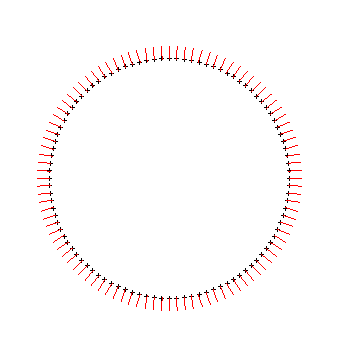
\includegraphics[scale=0.32]{2d/perimeter/circle-100-01-15-gradients}
        \subcaption{100 samples on a circle with $ r = 15 $}
        \label{fig:gradients_perimeter_2d_circle}
    \end{minipage}

    \begin{minipage}{0.8\linewidth}
        \centering
        \includegraphics[scale=0.32]{2d/perimeter/square-76-001-100}
        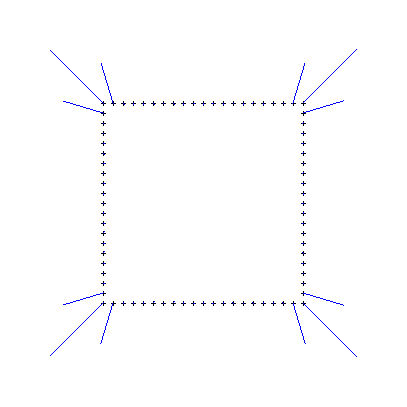
\includegraphics[scale=0.32]{2d/perimeter/square-76-001-100-gradients}
        \subcaption{76 samples on a square with $ r = 100 $}
        \label{fig:gradients_perimeter_2d_square}
    \end{minipage}

    \caption{Input point set / Computed gradients}
    \label{fig:gradients_perimeter_2d}
\end{figure}

In the previous screenshots, we can see that the gradients are (if the radius of
the balls are big enough and if the sampling is sufficiently uniform) in the
same direction that the normals to the underlying surface.

% TODO

\section{Relation with the mean curvature flow}

The flow we will obtain by considering the previously computed gradients will be
an approximation of the classical mean curvature flow.

Indeed, we will show that the norm of these gradients are estimations of the
mean curvature of the underlying sampled surface.

First, we will compute an approximation of the gradient of the area of the union
of balls.

% TODO

\begin{figure}[H]
    \centering
    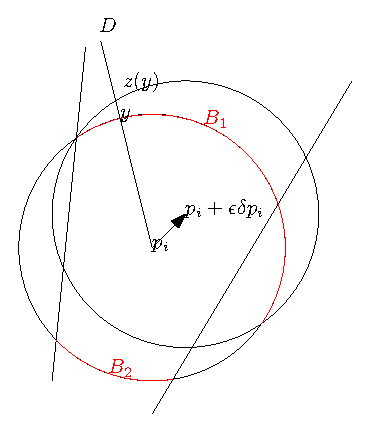
\includegraphics[scale=0.8]{2d/2d_proof_gradient_area_1}
    \caption{Situation for a ball $ B(x_i, r) $}
\end{figure}

Let's say that we move the point $ x _i $ by $ dx_i $, let's study the variation
of the area of $ V(x_i, X) \cap B(x_i, r) $.

If we denote the old area by $ A_{old} $ and the new area by $ A_{new} $, the we
have: $ A_{new} = A_{old} + A_1 - A_2 $ where $ A_1 $ is the upper gained area
and $ A_2 $ the lower lost area.

Then, we can approximate $ A_1 $ by $ \int_{B_1} || y - z(y) || dy $ where $ B =
\partial B_(x_i, r) \cap V(x_i, X) = B_1 \cup B_2 $ is the visible boundary of
the ball.

For any $ y \in B $, we define $ z(y) $ as the intersection of the half-line $ D $
with the circle of center $ x_i + dx_i $ with radius $ r $.
Then, we parametrize the half-line $ D $ by $ y + t \frac{y - x_i}{||y - x_i||}
$ where $ t \ge 0 $.

Let's find this intersection point by assuming that $ dx_i $ and $ t $ are small
such that $ t^2 = dx_i^2 = t \times dx_i = 0 $.

We need to find $ D \cap C(x_i + dx_i, r) $. Let $ t \ge 0 $ then , we have :
\begin{equation}
    || y + t \frac{y - x_i}{|| y - x_i||} - (x_i + dx_i) ||^2 = r^2
    \tag{$\star$}
\end{equation}

If we expand this expression, we get:

\begin{align*}
    (\star) & \iff || y
    - (x_i + dx_i) ||^2 + t^2 + 2t \left( \frac{y-x_i}{|| y - x_i||} | y - (x_i
        + dx_i) \right) = r^2 \\
    & \iff || y - x_i || ^2 - 2 (y - x_i | dx_i) + || dx_i || ^2 + t^2 + 2t
    \left( \frac{y-x_i}{|| y - x_i||} | y - (x_i + dx_i) \right) = r^2 \\
    & \iff -2 (y - x_i | dx_i) + 2t || y - x_i|| = 0 \\
    & \iff t = t^{\star} = \left( \frac{y - x_i}{||y - x_i||} | dx_i \right)
\end{align*}

Then, $ z(y) = y = t^{\star} \frac{y - x_i}{||y - x_i||} $ and $ || y - z(y) || =
t^{\star} $.

We deduce that :
$$ A_1 \approx \int_{B_1} \left( \frac{y - x_i}{||y - x_i||} | dx_i \right) dy $$
and:
$$ A_1 - A_2 \approx \int_{B} \left( \frac{y - x_i}{||y - x_i||} | dx_i \right) dy $$

Finally, we have:
\begin{equation}
    \label{eqn:gradient_area_2d}
    \partiald{A}{x_i} \approx \int_{B} \frac{y - x_i}{||y - x_i||} dy
\end{equation}

Now, let's find the link between the previously computed gradient and the mean
curvature. We suppose that our point cloud $ P $ is a sampling of an underlying
surface $ M $. More precisely, we suppose that $ P $ is an $ \epsilon $-sampling
of $ M $ defined in \cite{amenta1999surface}.

We will first do two approximations on \ref{eqn:gradient_area_2d}:
\begin{enumerate}
    \item the first one is to suppose that the offset of $ M $ is close enough to the offset of $ P $.
    \item the second one is that if the sampling is dense enough then we can replace $ p $
        by the projection of $ y $ on $ M $.
\end{enumerate}

Using these approximations, we get:
\begin{align*}
    \int_{\partial{P^r} \cap V(p, P)} (x - p) dx & \stackrel{(1)}{=} \int_{\partial{M^r} \cap V(p,
        P)} (x - p) dx \\
    &\stackrel{(2)}{=} \int_{\partial{M^r} \cap V(p, P)} (x - p_M(x)) dx \\
\end{align*}

Then, we will use the substitution $ q = p_M(x) \iff x = \phi(q) = q + \vec{n_M}(q) $
where $ \vec{n_M}(q) $ is the normal vector of $ M $ at $ q $ on the upper part
of $ \partial{M^r} \cap V(p, P) $.

We will need the Jacobian of this substitution. If we decompose this
substitution on $ T_p(M) \times [-r, r] $, where $ T_p(M) $ is the tangent space
of $ M $ at $ p $, we get: $ D \phi = id + r D \vec{n_M}(q) $.

Then, we use the fact that the matrix $ D \vec{n_M}(q) $ is diagonalizable and
that its eigenvalues are the principal curvatures.
We deduce that : $ \det (D \phi) = (1 + \kappa_1(q)) (1 + \kappa_2(q)) $.

Using an analogous substitution on the lower part of $ \partial{M^r} \cap V(p,
P) $, we get : $ \det (D \phi) = (1 - \kappa_1(q)) (1 - \kappa_2(q)) $.

By summing the two, we obtain: $ 2 (\kappa_1(q) + \kappa_2(q)) $.

It follows that:
\begin{align*}
    \int_{\partial{M^r} \cap V(p, P)} (x - p_M(x)) dx &= \int_{M \cap V(p, P)}
    r \times \vec{n_M}(q) ( \det (id + r D \vec{n_M}(q)) - \det (id - r D
    \vec{n_M}(q)) ) dq \\
    &= 2r \int_{M \cap V(p, P)} (\kappa_1(q) + \kappa_2(q)) \vec{n_M}(q) dq \\
\end{align*}

Finally, if we suppose that $ \vec{n_M}(q) = \vec{n_M}(p) $, $ \kappa_1(q) =
\kappa_1(p) $ and $ \kappa_2(q) = \kappa_2(p) $, we have the following final
result:

$$ \partiald{A}{p} = 2r (\kappa_1(p) + \kappa_2(p)) \vec{n_M}(p) \int_{M \cap V(p, P)} dq $$

In short, the gradient of the area of union of balls is proportional to the mean
curvature.

\section{Curvature estimation}

We can use the previous result to estimate mean curvature on a point set using
the norm of the gradients of the area of the union of balls.

We did our tests on a sampled ellipse with major / minor axes of $ a / b $. We
can parametrize this ellipse by :
\begin{cases}
    x(t) &= a \cos (t) \\
    y(t) &= b \sin (t)
\end{cases}

We recall the formula for computing the curvature of a parametrized curve:
$$ \kappa(t) = \frac{x'(t) y''(t) - y'(t) x''(t)}{(x'^2(t) +
    y'^2(t))^{\frac{3}{2}}} $$

For an ellipse, we obtain:
$$ \kappa(t) = \frac{ab}{(a^2 \cos^2(t) + b^2 \sin^2(t))^{\frac{3}{2}}} $$

We compare this for $ t = \frac{2 k \pi}{N} $ for $ k = 0 \ldots N - 1 $ with
the computed ones where $ N $ is the number of samples.

% TODO: pictures

\section{Gradient descent}

Then, as said in the introduction, we will approximate the mean curvature flow
by applying a gradient descent algorithm where the considered energy is the area
(or the perimeter of the boundary) of the union of balls.

This gradient descent will be done using a constant timestep (Euler explicit
scheme).

We needed to choose "good" weights for the gradient descent. Indeed, in a normal
mean curvature flow, all the points move with the same distance related to the
curvature. But here, this may not be the case since the energy depends on the
curvature of our restricted region.

One way to avoid this problem is to weight the gradient by the perimeter of the
visible part of the restricted region. But by doing that, we can divide by $ 0 $
so we need to choose the time step according to these weights in order to avoid
the case where a point does not see anything.

% TODO

\section{Experiments}

We did some experiments to validate our results: we first compared the two
gradient flows (area and perimeter of the boundary) to a set of points uniformly
sampled on an ellipse.

\begin{figure}[H]
    \centering

    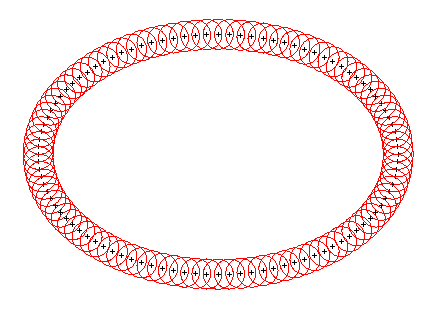
\includegraphics[scale=0.3]{2d/ellipse-balls-15}
    \subcaption{Minkowski sum of an ellipse and balls of radius $ 15 $}

    \includegraphics[scale=0.4]{2d/perimeter/ellipse-100-01-15}
    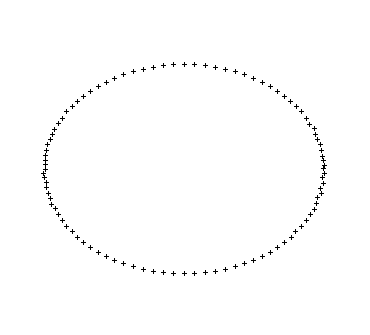
\includegraphics[scale=0.4]{2d/perimeter/ellipse-100-01-15-100}
    \subcaption{Perimeter flow : 0 / 100 iterations with a timestep of $ 0.5 $}
    \label{fig:ellipse_perimeter_flow}

    \includegraphics[scale=0.4]{2d/area/ellipse-100-01-15}
    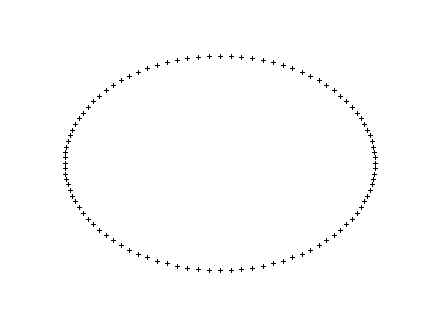
\includegraphics[scale=0.4]{2d/area/ellipse-100-01-15-100}
    \subcaption{Area flow : 0 / 100 iterations with a timestep of $ 0.1 $}
    \label{fig:ellipse_area_flow}
\end{figure}

Next, we add some outliers around the ellipse and observe the effects of the two
flows.

\begin{figure}[H]
    \centering

    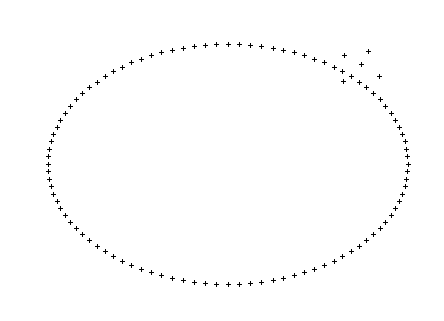
\includegraphics[scale=0.3]{2d/perimeter/ellipse-100-1-15-outliers}
    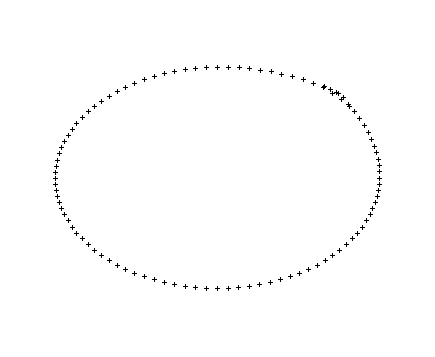
\includegraphics[scale=0.3]{2d/perimeter/ellipse-100-1-15-outliers-100}
    \subcaption{Perimeter flow : 0 / 100 iterations with a timestep of $ 1 $}
    \label{fig:ellipse_outliers_perimeter_flow}

    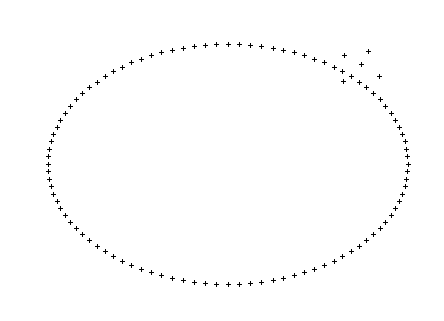
\includegraphics[scale=0.3]{2d/area/ellipse-100-01-15-outliers}
    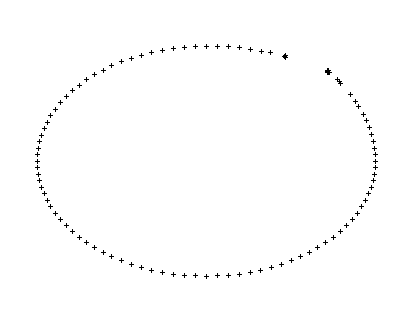
\includegraphics[scale=0.3]{2d/area/ellipse-100-01-15-outliers-40}
    \subcaption{Area flow : 0 / 40 iterations with a timestep of $ 0.1 $}
    \label{fig:ellipse_outliers_area_flow}
\end{figure}

Then, we added some Gaussian noise on these points to test the robustness of our
algorithm.

\begin{figure}[H]
    \centering

    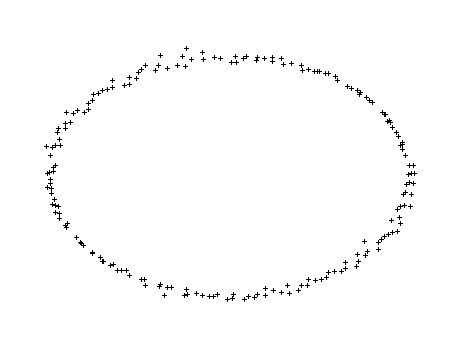
\includegraphics[scale=0.3]{2d/ellipse-noise-5-0}
    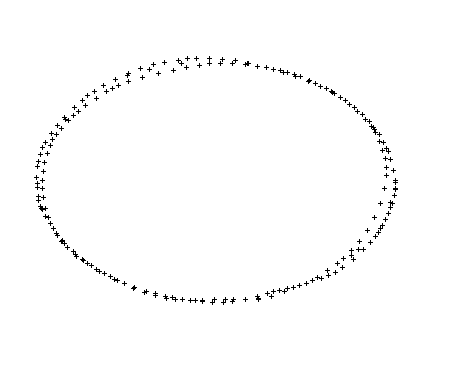
\includegraphics[scale=0.3]{2d/perimeter/ellipse-noise-5-75}
    \subcaption{Perimeter flow : 0 / 75 iterations with a timestep of $ 0.5 $}
    \label{fig:ellipse_noise_perimeter_flow}

    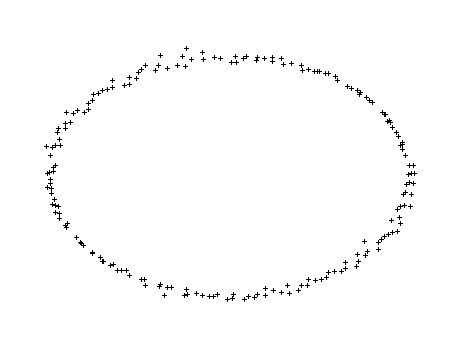
\includegraphics[scale=0.3]{2d/ellipse-noise-5-0}
    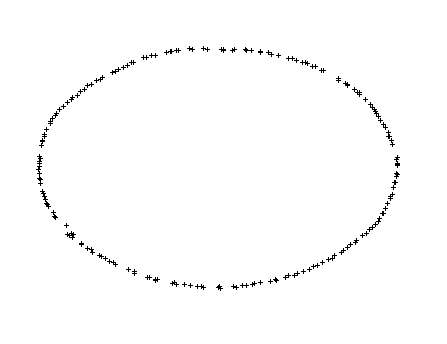
\includegraphics[scale=0.3]{2d/area/ellipse-noise-5-75}
    \subcaption{Area flow : 0 / 75 iterations with a timestep of $ 0.05 $}
    \label{fig:ellipse_noise_area_flow}
\end{figure}

We notice that the gradient flow of the area may create holes in the point set
which is not the case for the gradient flow of the perimeter.

On the contrary, the gradient flow of the perimeter of the boundary will smooth
the point set while redistributing the points in an uniform way.

% TODO: explain why
This can be explained by looking on a simple case with two intersecting balls:
\begin{itemize}
    \item for the area: TODO
    \item for the perimeter: the gradients are directed towards the outside
        and so the balls will be merged because we can say, using the triangle
        inequality, that in order to minimize the perimeter the balls must come
        closer.
\end{itemize}

The chosen radius will also influence the smoothing: points which are too far
away from other points (at distance greater than the radius) will not move. The
more the radius is big, the more points will move in big groups. Indeed, the
radius indicates how to take the neighbours of a point into account, the more
neighbours we take into account the more "global" the movement will be.

We also tried to add varying oscillations to our ellipse in order to see the
adaptive part of the algorithm. We generate oscillations with one or two
amplitudes.

For one constant amplitude:

\begin{figure}[H]
    \centering

    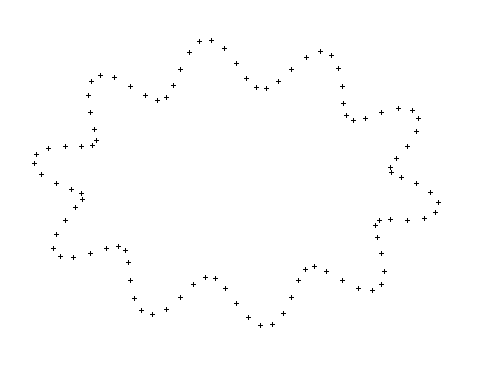
\includegraphics[scale=0.3]{2d/ellipse-osc-25-15-0}
    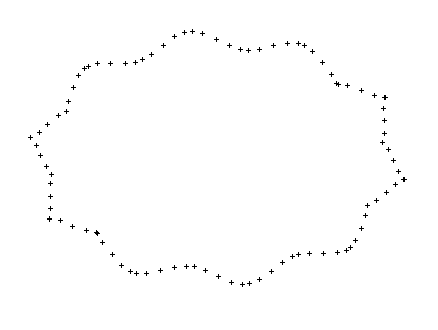
\includegraphics[scale=0.3]{2d/perimeter/ellipse-osc-25-15-50}
    \subcaption{Perimeter flow : 0 / 55 iterations with a timestep of $ 0.5 $
        and a radius of $ 15 $}
    \label{fig:ellipse_osc_perimeter_flow}

    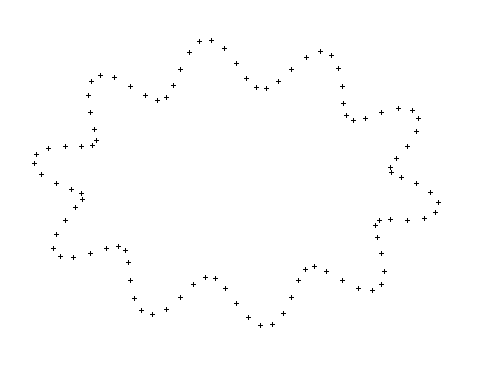
\includegraphics[scale=0.3]{2d/ellipse-osc-25-15-0}
    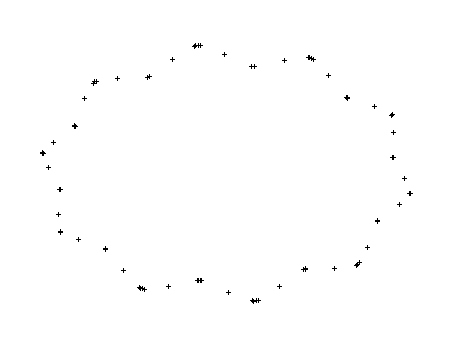
\includegraphics[scale=0.3]{2d/area/ellipse-osc-25-15-25}
    \subcaption{Area flow : 0 / 25 iterations with a timestep of $ 0.05 $ and a
        radius of $ 15 $}
    \label{fig:ellipse_osc_area_flow}
\end{figure}
% TODO: remove extra space

For two different amplitudes:

\begin{figure}[H]
    \centering

    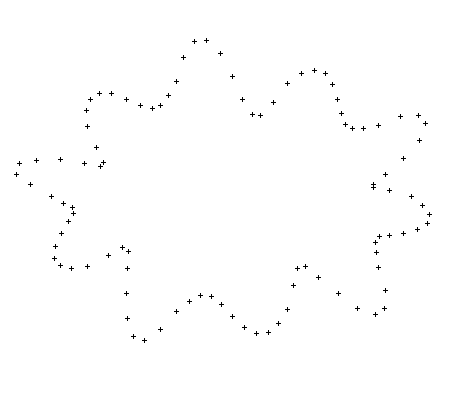
\includegraphics[scale=0.3]{2d/ellipse-osc2-20}
    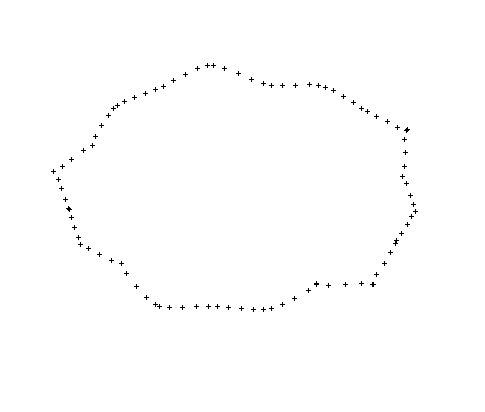
\includegraphics[scale=0.3]{2d/perimeter/ellipse-osc2-20-15-55}
    \subcaption{Perimeter flow : 0 / 55 iterations with a timestep of $ 0.5 $
        and a radius of $ 15 $}
    \label{fig:ellipse_osc2_perimeter_flow}

    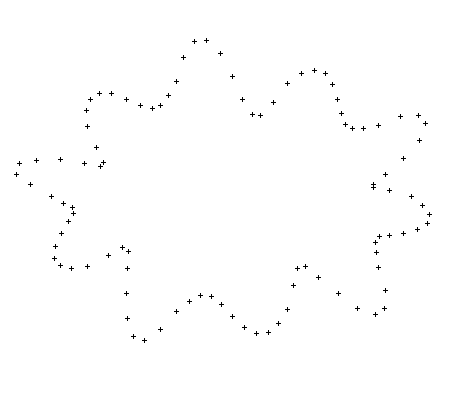
\includegraphics[scale=0.3]{2d/ellipse-osc2-20}
    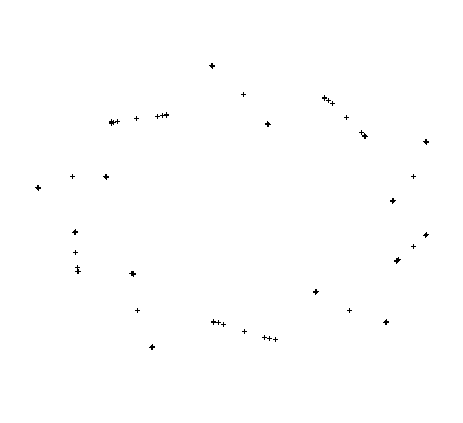
\includegraphics[scale=0.3]{2d/area/ellipse-osc2-20-15-25}
    \subcaption{Area flow : 0 / 25 iterations with a timestep of $ 0.05 $ and a
    radius of $ 15 $}
    \label{fig:ellipse_osc2_area_flow}
\end{figure}
% TODO: remove extra space

% TODO: explain why

An other experiment we did is to take points on a line segment and to fix its
endpoints. Then, we apply our flow on this point set. We expect the flow to
smooth the point set: points should get closer and closer to an uniformly
sampled set of points.

\begin{figure}[H]
    \centering

    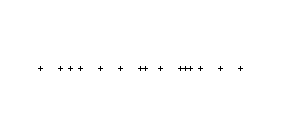
\includegraphics[scale=0.5]{2d/perimeter/line-05-15-0}
    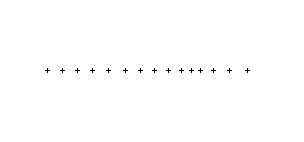
\includegraphics[scale=0.5]{2d/perimeter/line-05-15-50}
    \subcaption{Perimeter flow : 0 / 50 iterations with a timestep of $ 0.5 $}
    \label{fig:line_fixed_perimeter}

    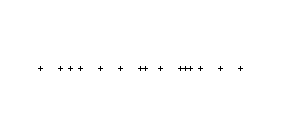
\includegraphics[scale=0.5]{2d/area/line-01-15-0}
    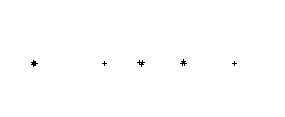
\includegraphics[scale=0.5]{2d/area/line-01-15-50}
    \subcaption{Area flow : 0 / 50 iterations with a timestep of $ 0.1 $}
    \label{fig:line_fixed_area}
\end{figure}

% TODO: explain why

% Union of balls
% Intersection with Voronoi cells
% Volume
% Gradient descent: weights
% Experiments

% vim: set spelllang=en :


\backmatter
% \appendix

% Bibliography
\bibliographystyle{plain}
\bibliography{bibfile}

\end{document}

